\documentclass[12pt]{article}
\usepackage{graphicx,import}
\usepackage[svgnames]{xcolor} 
\usepackage{fancyhdr}
\usepackage{subfig}
\usepackage{hyperref}
\usepackage{enumitem}
\usepackage{cite}
\usepackage[many]{tcolorbox}
\usepackage{listings }
\usepackage[a4paper, total={6in, 8in} , bottom = 25mm , top = 25mm, headheight = 1.25cm , includehead,includefoot,heightrounded ]{geometry}
\usepackage{afterpage}
\usepackage{amssymb}
\usepackage{pdflscape}
\usepackage{gensymb}
\usepackage{textcomp}
\usepackage{xecolor}
\usepackage{rotating}
\usepackage{pdfpages}
\usepackage[Kashida]{xepersian}
\usepackage[T1]{fontenc}
\usepackage{tikz}
\usepackage[utf8]{inputenc}
\usepackage{PTSerif} 
\usepackage{seqsplit}

\usepackage[edges]{forest}

\usepackage{listings}
\usepackage{xcolor}

\hypersetup{
	colorlinks   = true, %Colours links instead of ugly boxes
	urlcolor     = blue, %Colour for external hyperlinks
	linkcolor    = blue, %Colour of internal links
	citecolor   = red %Colour of citations
}
 
\definecolor{codegreen}{rgb}{0,0.6,0}
\definecolor{codegray}{rgb}{0.5,0.5,0.5}
\definecolor{codepurple}{rgb}{0.58,0,0.82}
\definecolor{backcolour}{rgb}{0.95,0.95,0.92}
 
\NewDocumentCommand{\codeword}{v}{
\texttt{\textcolor{blue}{#1}}
}
\lstset{language=java,keywordstyle={\bfseries \color{blue}}}

\lstdefinestyle{mystyle}{
    backgroundcolor=\color{backcolour},   
    commentstyle=\color{codegreen},
    keywordstyle=\color{magenta},
    numberstyle=\tiny\color{codegray},
    stringstyle=\color{codepurple},
    basicstyle=\ttfamily\normalsize,
    breakatwhitespace=false,         
    breaklines=true,                 
    captionpos=b,                    
    keepspaces=true,                 
    numbers=left,                    
    numbersep=5pt,                  
    showspaces=false,                
    showstringspaces=false,
    showtabs=false,                  
    tabsize=2
}

\lstset{style=mystyle}

\settextfont[Scale=1.2 ,BoldFont={Bahij Nazanin-Bold.ttf} , ItalicFont = {IRNazaninIranic.ttf}]{Bahij Nazanin-Regular.ttf}
\setlatintextfont[Scale = 1.0]{Garamond}
\DefaultMathsDigits 
\DeclareMathSizes{11}{19}{13}{9} 
%\DeclareMathSizes{12}{14.4}{8}{9}





\newenvironment{changemargin}[2]{%
\begin{list}{}{%
\setlength{\topsep}{0pt}%
\setlength{\leftmargin}{#1}%
\setlength{\rightmargin}{#2}%
\setlength{\listparindent}{\parindent}%
\setlength{\itemindent}{\parindent}%
\setlength{\parsep}{\parskip}%
}%
\item[]}{\end{list}}


\definecolor{foldercolor}{RGB}{124,166,198}

\tikzset{pics/folder/.style={code={%
    \node[inner sep=0pt, minimum size=#1](-foldericon){};
    \node[folder style, inner sep=0pt, minimum width=0.3*#1, minimum height=0.6*#1, above right, xshift=0.05*#1] at (-foldericon.west){};
    \node[folder style, inner sep=0pt, minimum size=#1] at (-foldericon.center){};}
    },
    pics/folder/.default={20pt},
    folder style/.style={draw=foldercolor!80!black,top color=foldercolor!40,bottom color=foldercolor}
}

\forestset{is file/.style={edge path'/.expanded={%
        ([xshift=\forestregister{folder indent}]!u.parent anchor) |- (.child anchor)},
        inner sep=1pt},
    this folder size/.style={edge path'/.expanded={%
        ([xshift=\forestregister{folder indent}]!u.parent anchor) |- (.child anchor) pic[solid]{folder=#1}}, inner xsep=0.6*#1},
    folder tree indent/.style={before computing xy={l=#1}},
    folder icons/.style={folder, this folder size=#1, folder tree indent=3*#1},
    folder icons/.default={12pt},
}

\begin{document}


%%% title pages
\begin{titlepage}
\begin{center}
        
\vspace*{0.7cm}


\includegraphics[width=0.4\textwidth]{sharif1.png}\\
\vspace{0.5cm}
\textbf{ \Huge{\emph ‌اندازه‌گیری و کنترل کامپیوتری} }\\
\vspace{0.5cm}
\textbf{ \Large{ تمرین اول} }
\vspace{0.2cm}
       
 
      \large \textbf{دانشکده مهندسی کامپیوتر}\\\vspace{0.2cm}
    \large   دانشگاه صنعتی شریف\\\vspace{0.2cm}
       \large   ﻧﯿﻢ سال دوم 00-99 \\\vspace{0.2cm}
      \noindent\rule[1ex]{\linewidth}{1pt}
استاد:\\
    \textbf{{جناب آقای دکتر همت‌یار}}


    \vspace{0.15cm}
نام و نام خانوادگی:\\

       
    \textbf{{امیرمهدی نامجو - 97107212}}
\end{center}
\end{titlepage}
%%% title pages


%%% header of pages
\newpage
\pagestyle{fancy}
\fancyhf{}
\fancyfoot{}
\cfoot{\thepage}
\chead{تمرین اول}
\rhead{
\includegraphics[width=0.1\textwidth]{sharif.png}}
\lhead{امیرمهدی نامجو}
%%% header of pages

\KashidaOff


\section*{سوال 4}

\begin{center}
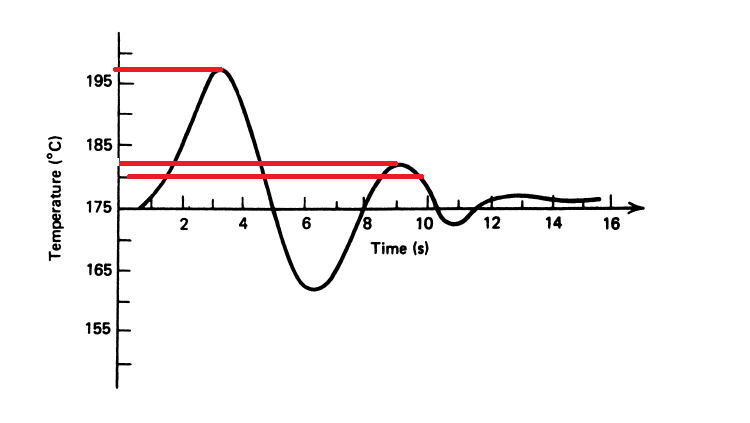
\includegraphics[width = 1.0 \textwidth]{images/1.png}
\end{center}

مطابق شکل، بیشنه مقدار تقریبا در $197$ درجه اتفاق می‌افتد. پس بیشینه خطا

$$197 - 175 = 22 \degree C $$

است. همچنین برای زمان Settling، از آن جایی که بازه انحراف بین $180$ تا $170$ درجه سانتی گراد است، اولین جایی که این درجه رد شده است، حدود $1.5$ و اولین جایی که بعد از آن استیبل شده و از این بازه خارج نشده است، در  $9.8$ ثانیه است. پس جواب

$$9.8 - 1.5 = 8.3 s$$
است.


\section*{سوال 5}


\begin{center}
	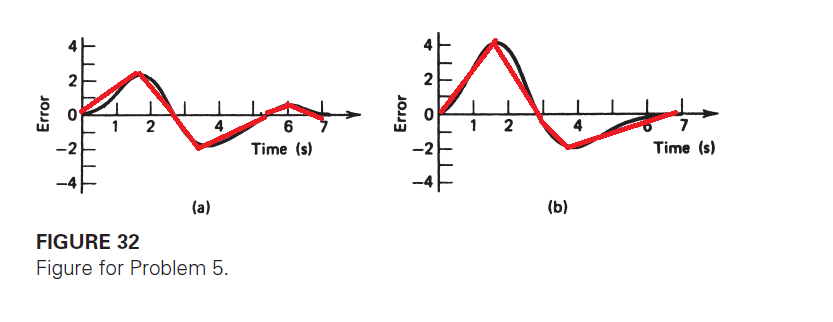
\includegraphics[width = 1.0 \textwidth]{images/2.png}
\end{center}


با توجه به این مثلث بندی تقریبی، مساحت را تخمین می زنیم.

$$S_a = (2 \times (2.6) + 2 \times (5.2 - 2.6) + 1 \times (7 - 5.2) ) /2 = 6.1$$

$$S_b =  ((4 \times 3) + 2 \times (7-3)) / 2 = 10$$

با توجه به این که اختلاف بدست آمده هم زیاد است، مشخصا (و حتی به شکل چشمی) مساحت a از b کمتر است. بنابراین جواب سوال a است.

\section*{سوال 6}

$$a_3 =  \frac{1}{4} (a_2) = \frac{1}{4} (4.4 \%) = 1.1 \%$$



\section*{سوال 7}

اختلاف قله اول با معیار
$197 - 175 = 22$
است. در نتیجه قله دوم باید حدود $5.5$ فاصله داشته باشد ولی حدودا
$182 - 175 = 7$
است. قله بعدی حدودا $178$ یا $177$ است که می شود $2$ یا $3$ در حالی که اگر براساس $7$ قبلی در نظر بگیریم باید $1.75$ می بود. در نتیجه در هر مرحله شاهد این هستیم که قله ها از مقدار روش quarter-amplitude بیش تر است و یعنی این نمودار با این معیار تطابق ندارد.


\section*{سوال 8}


$$50 mA \times \frac{225 m^3/h}{300 m^3/h} =  37.5 mA$$

\section*{سوال 9}

$$(16)_{10} = (10000)_2$$

\section*{سوال 10}

\subsection*{a}

با توجه به این که مقیاس $0.15m$ است، پس ارزش ارقام به ترتیب از LSB به MSB به صورت $0.15$ - $0.30$ - $0.6$ و $1.2$ است.

$$1.7 - 1.2 = 0.5 \rightarrow 1$$
$$0.5 < 0.6 \rightarrow 0$$
$$0.5 - 0.3 = 0.2 \rightarrow 1$$
$$0.2 - 0.15 = 0.05 \rightarrow 1$$

$$1.7 \rightarrow 1011$$

راه دیگر تشکیل جدول به ازای همه مقادیر بود که ببینیم به کدام یک نزدیک‌تر است. همچنین می‌شد بگوییم که $1011 = 1.65$ و $1100 = 1.8$ و چون هنوز به $1.8$ نرسیده است، شاهد تغییر بیت نخواهیم بود و معادل با نمایش $1.65$ خواهد بود.
\subsection*{b}

$$1000 = 1.2$$

$$1001 = 1.35$$

پس اگر عدد $1000$ باشد جواب می تواند هر عددی بین $1.2$ تا $1.35$ باشد.

\section*{سوال 15}

\begin{latin}
1 lb-force = 4.44822  Newton
1 inch = 0.0254 meter
\end{latin}

$$14.7 lb/in^2 = 14.7 lb/in^2 \times 4.4482 N/lb \times (1/0.0254 in/m)^2 = 101352.43 Pa$$

البته خود کتاب هم ضریب تبدیل دیگری ارائه داده که با استفاده از آن می شود:

$$14.7 \times (6895) = 101356 Pa $$

\section*{سوال 16}


\subsection*{a}
$$a= \frac{0.25 mi \times 5280 ft/mi}{ (7.2 s)^2 } \times 2 = 50.93 ft/s^2$$


\subsection*{b}
$$50.93 ft/s^2 \times 0.3048 m/ft = 15.52 m/s^2 $$

\subsection*{c}

$$v = \sqrt{2 \times 0.25 mi \times 1609.34 m/mi \times 15.52 m/s^2} = 111.7 m/s$$
\subsection*{d}

$$W = \frac{( 111.7 m/s)^2 \times (2000 lb \times 0.4535 kg/lb)}{2} = 5.658 \times 10^6 J$$


\section*{سوال 17}

$$L = a P + b$$

$$5.5 = 3a+b  $$
$$8.6 = 15a + b$$


$$a = \frac{31}{120} psi/m , b= \frac{189}{40} m$$

برای قسمت اول، داریم:

$$P  = (7.2 - \frac{189}{40}) \times \frac{120}{31} \approx 9.58 psi $$

برای قسمت دوم، داریم:

$$L =\frac{31}{120} \times 4.7 + \frac{189}{40} =5.939 m \approx 5.94 m $$


\section*{سوال 18}

قسمت اول
$$Q = 45 \sqrt{(12 - 2)} =142.3 gal/min $$


قسمت دوم:

$$162 = 45 \sqrt{I -2} \rightarrow I = (162/45)^2 + 2 = 14.96 mA$$



\section*{سوال 19}

$$1500 \times (\pm 0.005) = \pm 7.5 \Omega$$

$$397 \Omega \pm 7.5 \Omega = [389.5\Omega , 404.5\Omega]$$


\section*{سوال 20}

$$0.5 mV/\degree C \pm 1\% = 0.5 mV/\degree C \pm 0.005 mv/\degree C  = (0.495 mV/\degree C , 0.505 mv/\degree C)$$

$$60 \degree C \times 0.5 mV/\degree C = 30 mV$$
$$60 \degree C \times 0.495 mV/\degree C = 29.7 mV$$
$$60 \degree C \times 0.505 mV/\degree C = 30.3 mV$$

پس ولتاژ در بازه
 $30 mV \pm 3 mV$
  خواهد بود.




\section*{سوال 26}
$$T = T_i + (T_f - T_i) \times (1 - e^{-t / \tau})$$

$$
\begin{array}{l}
	t=0.5 \mathrm{~s} ; T=22+28\left(1-\mathrm{e}^{-0.5 / 3.3}\right)=25.9 \degree \mathrm{C} \equiv 3.885 mv \\
	t=2.0 \mathrm{~s} ; T=22+28\left(1-\mathrm{e}^{-2 / 3.3}\right)=34.7 \degree \mathrm{C} \equiv 5.205 mv \\
	t=3.3 \mathrm{~s} ; T=22+28\left(1-\mathrm{e}^{-3.3 / 3.3}\right)=39.7 \degree \mathrm{C} \equiv 5.955 mv \\
	t=9.0 \mathrm{~s} ; T=22+28\left(1-\mathrm{e}^{-9 / 3.3}\right)=48.2 \degree \mathrm{C} \equiv 7.23 mv
\end{array}
$$

برای معادل سازی با میلی‌ولت، عدد درجه سانتی گراد در تابع انتقال استاتیک ($0.15 mV / \degree C$) ضرب شده است.


\section*{سوال 27}

$$52 = 44 + (70 - 44)(1 - e^{- 4.5 / \tau}) $$

$$\frac{8}{26} =(1 - e^{- 4.5 / \tau}) \rightarrow \frac{-4.5}{\tau}= \ln (\frac{18}{26}) \rightarrow \tau = 12.237 s $$

\section*{سوال 28}

از آن جایی که عبارت
$1 - e^{-t / \tau}$
در اصل کسری از مقدار تغییرات که اضافه شده است را نشان می دهد و این جا هم حرکت از $0$ شروع شده داریم:

$$t= 1 - e^{-t / 35} = 0.8 \rightarrow -t/35 = \ln (0.2) \rightarrow t = 56.33 ms$$



\section*{سوال 29}

$$4.00 V / (20  \times 10^{-3} V/kPa) = 200 kPa$$

$$200 = 100 + (400 - 100)(1 - e^{-t/4.9}) \rightarrow \frac{1}{3} = (1 - e^{-t/4.9})$$
$$-t/4.9 = \ln(\frac{2}{3}) \rightarrow t = 1.986 s \approx 1.99 s$$

\section*{سوال 30}

\subsection*{a}
$$p = 40 + (150 - 40) \times (1 - e^{-0.5/0.350 }) \approx 123.6 kPa$$

$$R = 0.15 \times 123.6 +2.5 =  21.04 k\Omega$$

$$V = \frac{10 \times 21.04 k}{21.04 k + 10k} = 6.77 V $$

\subsection*{b}

$$5 = \frac{10 R}{R + 10 k} \rightarrow R = 10 k\Omega$$

$$10 k\Omega = 0.15 (k\Omega/psi)P + 2.5 k\Omega \rightarrow P = 50 psi $$

$$t= 50 = 40 + (150 -40) \times (1 - e^{-t/0.350 }) \rightarrow -t/0.35 = \ln(10/11) = 0.033 s$$


\section*{سوال 32}

مقدار تئوری:

$$I = V/R = 4.7 / 1.5k = 3.13333333 mA = 3.1\bar{3} mA$$ 

که این مقدار دقیق است و  می‌توان بی‌نهایت رقم با معنا برای آن در نظر گرفت. (یا تا هر تعدادی که سیستم محاسبه ما نظیر ماشین‌حساب و کامپیوتر می‌تواند ذخیره کند)


مقدار در عمل:

$$I = V/R = 4.7 / 1.5k = 3.1 mA$$

چون دو کمیت دیگر دو رقم با معنا داشتند، کمیت I هم باید دو رقم با معنا داشته باشد.


\section*{سوال 33}

$$10.1 + 12.2 + 9.7 + 8.8 + 11.4 + 12.9 + 10.2 + 10.5 + 9.8 + 11.5 +$$
$$10.3 + 9.3 + 7.7 + 10.2 + 10.0 + 11.3 = 165.9$$

$$Mean: 165.9 / 16 = 10.36875 gal/min$$


$$Var = \sum((x_i - 10.36875)^2)/15 = 1.65029$$
$$StdDev = \sqrt{Var} = 1.284636$$


برای واریانس و انحراف از معیار،‌ از فرمول واریانس نمونه (که تقسیم بر $n-1$ می‌کند) استفاده شده است.

برای چک کردن جواب هم از کد صفحه بعد در زبان R استفاده شده است:

\begin{latin}
\begin{lstlisting}[language=R]
	x = c(10.1 , 12.2 , 9.7
	, 8.8 , 11.4 , 12.9 
	,10.2 , 10.5 , 9.8 , 11.5 , 10.3 , 9.3 , 7.7 , 10.2 , 10.0 , 11.3)
	m<-mean(x)
	v <- var(x)
	stdd <- sqt(v)
	
\end{lstlisting}
\end{latin}


\section*{سوال 34}

\subsection*{a}
$$V_i = (45 mV/kPa \pm 5\% ) \times 20 kPa = 0.9V \pm 0.045V = (0.855V , 0.945V) $$

$$V_f = (45 mV/kPa \pm 5\% ) \times 100 kPa = 4.5V \pm 0.225V = (4.275V , 4.725V) $$

\subsection*{b}

$$V = V_i + (V_f - V_i)(1 - e^{-t / \tau}) $$
$$V = (45 \pm 5\% ) (20 + 80 (1 - e^{-t /(4 \pm 0.4)}))$$


چون مقادیر $P$ را دقیق می‌دانستیم ولی $V$ ها حالت‌های زیادی پیدا می‌کرد بسته به مثبت و منفی بودن، از $P$ استفاده می‌کنیم.

اگر $\tau = 4.4$ بگیریم داریم
$(1 - e^{-2 /(4.4)}) = 0.36526$

اگر $\tau = 3.6$ بگیریم داریم:
$(1 - e^{-2 /(3.6)}) = 0.426247$

در حالت اول، مقدار کمینه $45 \pm 5\%$ را می‌گذاریم که کمترین مقدار و در حالت دوم مقدار بیشینه را می‌گذاریم که بیش‌ترین مقدار $V$ را به دست آوریم:

$$V_{max} = 47.25 mV/kPa \times (20+80*0.426247) kPa = 2.55621 V \approx 2.556 V$$

$$V_{min} = 42.75 mV/kPa \times (20+80*0.36526) kPa = 2.10419 V \approx 2.104 V$$

که این به نوعی برابر است با
 $2.330 V \pm 0.226 V$


\end{document}



